% Tento soubor nahraďte vlastním souborem s obsahem práce.
%=========================================================================
% Autoři: Michal Bidlo, Bohuslav Křena, Jaroslav Dytrych, Petr Veigend a Adam Herout 2019

% Pro kompilaci po částech (viz projekt.tex), nutno odkomentovat a upravit
%\documentclass[../projekt.tex]{subfiles}
%\begin{document}

\chapter{Úvod}
\label{uvod}
Data a informace dnes představují jeden z nejcennějších zdrojů moderní společnosti. Často jsou označována jako "digitální zlato", protože jejich správné 
využití může přinést obrovskou hodnotu v různých oblastech – od vědy a průmyslu až po zdravotnictví a každodenní život. Aby však mohla být efektivně využita, 
je nutné je správně zaznamenávat, ukládat a analyzovat.

Vzhledem k široké škále oblastí, kde data vznikají, se používají různé metody jejich sběru a uchovávání. Data mohou pocházet z různých zdrojů – například 
senzorů měřících fyzikální veličiny, síťových zařízení sledujících internetový provoz, medicínských přístrojů monitorujících životní funkce pacientů, 
ekonomických systémů analyzujících finanční transakce či průmyslových strojů zaznamenávajících provozní parametry. Každý z těchto zdrojů má specifické 
požadavky na způsob sběru, formátování a uchovávání dat. 

Tato bakalářská práce je věnována návrhu a implementaci takového zařízení, které bude schopno záznamu dat. Požadavek na zařízení vznikl od firmy NXP 
Semiconductors, konkrétně od týmu zaměřeného na bezdrátové nabíjení, ve kterém pracuji. Tento tým působí v České republice – v pobočkách v Brně a Rožnově 
pod Radhoštěm – a zároveň má své zastoupení v Asii a Severní Americe. NXP Semiconductors je jedním z předních členů WPC (Wireless Power Consortium), 
organizace zodpovědné za definování standardu Qi pro bezdrátové nabíjení. Primární zaměření NXP v této oblasti spočívá ve vývoji referenčních designů 
pro automotive sektor, kde zákazníkům poskytuje řešení určená pro integraci do vozidel.

Zákazníci, kteří využívají referenční designy NXP, pocházejí z celého světa a dostávají téměř hotový produkt, který lze následně certifikovat v Qi 
certifikačních laboratořích. Nicméně i přesto, že jsou referenční designy navrženy podle nejnovějších standardů, často dochází k jejich úpravám podle 
specifických požadavků zákazníků, zejména s ohledem na konkrétní poptávku koncového zákazníka (OEM – Original Equipment Manufacturer). Tyto požadavky 
jsou obvykle shrnuty v RFQ (Request for Quotation), kde zákazník specifikuje konkrétní požadavky na systém. Tyto úpravy mohou být například realizovány 
z důvodu snížení ceny nebo zlepšení výkonu, například EMC charakteristik a nebo speciální chování bezdrátové nabíječky v krajních situacích. 

Při jakýchkoli úpravách však vznikají nové technické výzvy, a proto NXP poskytuje zákazníkům plnou technickou podporu až do úspěšné certifikace. Certifikace 
probíhá v různých laboratořích po celém světě, avšak ne vždy může být přítomen zaměstnanec NXP, který by dohlížel na celý proces a zajistil, že certifikace 
proběhne hladce. V těchto případech se tým pro bezdrátové napájení momentálně spoléhá pouze na záznamy poskytnuté operátorem certifikační laboratoře. 
Tyto záznamy však pocházejí pouze ze strany přijímače – tedy certifikačního zařízení, zpravidla od výrobců Nok9 nebo Granite River Labs (GRL). Ty poskytují 
některé z důležitých informací, bohužel ale tyto nabídnuté záznamy nezahrnují explicitní informace o chování vysílače. Pokud tedy bezdrátová nabíječka, tedy 
vysílač nějakým testem neprojde, což se občas stává, je často náročné zpětně identifikovat příčinu problému. \cite{nxp_wireless_charging_team}


\chapter{Záznam dat}
\label{zaznam_dat}

\label{uvod}

\section{Počátky záznamu a zpracování dat (Historie záznamu a zpracování dat - předchozí název)}
\label{historie}
Lidstvo již od svých počátků potřebovalo zaznamenávat data, neboť člověk mnohdy dokáže datům přiřadit sémantiku - tedy význam, a proměnit je tak v informace. 
Právě díky nim se lidé mohou učit z minulých zkušeností, předávat znalosti dalším generacím, organizovat společenské a obchodní procesy a podporovat rozvoj 
vědy a technologií. Proto se již od pravěku hledaly způsoby, jak evidovat důležité události a hodnoty. První formy záznamu dat sahají až 19 tisíc let před 
Kristem, kdy v paleolitu vznikl nástroj známý jako kost Ishango. Tento jednoduchý nástroj, vyrobený z kosti paviána, obsahoval vyryté zářezy, které 
pravděpodobně sloužily k provádění základních matematických operací, jako je sčítání či násobení.

\begin{figure}[h] % obrazek ishango
    \centering
    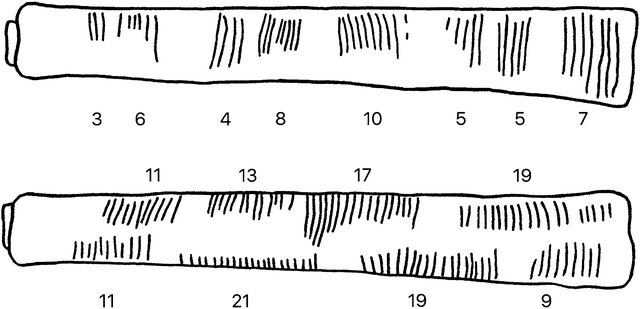
\includegraphics[width=0.6\textwidth]{obrazky-figures/ishango.jpg}
    \caption{Kost Ishango sloužící k záznamu informací v době Paleolitu \cite{ishango_picture}}
    \label{fig:ishango}
\end{figure}

S příchodem prvních civilizací se začaly vyvíjet lepší metody uchovávání dat. Ve starověké Mezopotámii, oblasti mezi řekami Eufrat a Tigris, kde sídlil národ 
Sumérů, vzniklo kolem roku 3400 před naším letopočtem klínové písmo. Tento typ písma byl využíván hlavně pro zápis obchodních transakcí, zákonů a dalších 
důležitých informací, které byly zaznamenávány na hliněné tabulky pomocí rákosového stylusu. O několik století později, kolem roku 3200 př. n. l., začali 
Egypťané používat hieroglyfy, které byly ryty do kamene nebo zapisovány na papyrus, což umožnilo uchovávat důležité administrativní a náboženské záznamy. 
V Číně se mezi 1200–1000 př. n. l. používaly věštecké kosti, na které se zaznamenávaly otázky kladené orákulu - což jsou důležité otázky, zejména ve věcech 
budoucnosti, i jeho odpovědi, čímž vznikly první organizované záznamy psané ranými čínskými znaky.

\newpage

Průlomem pro zaznamenáváním dat, bylo vynalezení knihtisku, které vymyslel Johann Gutenberg ve 40. letech 15. století. Do této doby byly informace 
zaznamenávány ručním přepisováním, což bylo zdlouhavé a nákladné. V počátcích měl knihtisk význam převážně z náboženského hlediska, díky tisku se Bible mohla 
šířit mezi širokou veřejností, což přispělo k protestantské reformaci a změně křesťanského světa. Nicméně knihtisk obecně změnil způsob, jakým lidé přistupují 
k informacím a učinil je dostupnějšími. \cite{knihtisk_medium}

V 17. století se dále pokročilo, jak v způsobech záznamu dat, tak i s jejich zpracováním. Významným představitelem tohoto období je John Graunt, jež se 
věnoval studiu dat o úmrtnosti v Londýně, během čehož odhalil určité opakující se vzorce a zákonitosti na základě, kterých položil základy moderní statistiky. 
V následujících staletích pokračoval vývoj metod pro práci s daty, zejména díky rozvoji matematiky, fyziky a statistiky. \cite{britanicca_John_Graunt}
% Jako hlavni predstavitele tohoto obdobi lze uvest jmena jako Bayes, Laplace, Pierre-Simon, Carl Friedrich Gauss, Galton
\section{Záznam a zpracování dat v moderní době}
% TODO: pocet normostran (cca 3.1)
S pokročilými metodami na zpracování dat, také rostly nároky na výpočty a vznikla tak potřeba efektivnějších nástrojů pro zisk a analýzu dat. S tímto rozvojem 
souvisí i technologický pokrok v oblasti záznamu dat, který prošel dlouhou cestou – od jednoduchých mechanických přístrojů přes magnetické pásky až po moderní 
digitální záznamníky schopné uchovávat a analyzovat obrovské objemy informací v reálném čase.

%\section{Možnosti záznamu dat}
%\label{moznosti_zaznamu_dat}
  
\subsection{Analogový záznam dat} %TODO: zde popsat i analogový záznam i digitální záznamníky
\label{moznosti_zaznamu_dat}
Prvními specializovanými záznamníky byly mechanické či elektromechanické (analogové) zařízení, ty primárně sloužily k zaznamenávání fyzikálních veličin, 
jako je například teplota, tlak, vlhkost nebo vibrace. Ty využívaly myšlenky mechanického pohyblivého pera, které převádělo naměřenou hodnotu fyzikální 
veličiny na samočinný pohyb. Aby tento mechanický pohyb mohl být uskutečněn, bylo třeba nejprve hodnotu měřené veličiny, například pro měření teploty, lze 
využít bimetalový pásek, který je složen ze dvou kovových materiálů s různou hodnotou teplotní roztažitelnosti. Pokud následně dojde ke změně teploty, způsobí 
tento přechodný jev pohyb kovového pásku, a ten je následně převeden na pohyb mechanického pera.

% mechanicky -< samocinny
% pomocí kterého se zapisovala změřená hodnota na paměťové médiu (papírová páska nebo papírový buben)

\begin{figure}[h] % obrazek polygraf
    \centering
    \includegraphics[width=0.50\textwidth]{obrazky-figures/polygraaf.png}
    \caption{Ukázka zařízení patřící do skupiny analogových záznamníků - polygraf \cite{polygraph_picture}}
    \label{fig:polygraaf}
\end{figure}

Mezi přístroje využívající principu analogového záznamu, patří například polygraf - využívající se například jako detektor lži, cirkulární grafový záznamník 
(Circular Chart Recorder) využívající se pro měření teploty.


\section{Digitální záznamová jednotka (datalogger)}
\label{digitalni_zaznamnik}
Co je to digitální záznamník + jak zaznamnik realizovat jestli PC nebo MCU (dedikovane zarizeni)

\begin{figure}[h] % obrazek polygraf
    \centering
    \includegraphics[width=0.95\textwidth]{obrazky-figures/common_digital_datalogger_scheme.png}
    \caption{Obecné schéma digitálního záznamníku}
    \label{fig:polygraaf}
\end{figure}
vstupy -> surové data (raw data)

vystupy -> organizovaná data např. v textové podobě

\subsection{Digitální záznamník v počítačovém systému}
K cemu jsou vyuzivany digitalni zaznamniky na PC.

\subsection{Digitální záznamník na platformě mikrořadiče}

\section{Koncepty využívané ke zpracování dat digitálních záznamníků}
cirkulární buffer, vícenasobná vyrovnávací paměť (multiple-buffering), dávkové ukládání/zpracování (batch processing), nízko-energetické režimy 
(low-power modes)


\chapter{Návrh digitálního záznamníku}

\section{Představení existujících řešení}

\section{Výběr vhodné platformy}
Neni vhodne implementovat zaznamnik na pocitacovem systemu, je treba zvolit stragii implementace na mikroradici, porovnat FRDM-MCXN947, STM32 a ESP32. 

Pripraven i popis jadra ARM Cortex-M33, ktere vyuziva FRDM-MCXN947.

\section{Možnosti způsobu ukládání získaných dat}

% ----------------------------------------------------
% DALSI NAZVY: Volba datového úložiště, Výběr externího uložiště pro záznam dat
\section{Výběr úložiště pro záznam dat}
Obecný popis, proč je potřeba externí uložiště, že by se data mohla ukládat i v RAM paměti, ale že by tam moc dlouho nevydržela, 

\subsection{SDHC karta}

\subsection{Quad-SPI flash}

\subsection{USB flash disk}

% ----------------------------------------------------
% DALSI NAZVY: Volba datového úložiště, Výběr externího uložiště pro záznam dat
\section{Možnosti správy dat - souborové systémy} 
Obecný popis, souborový systém je zodpovědný za organizaci, správu a přístup k datům na zvoleném úložném médiu.

\subsection{FATFS}

\subsection{Chan FATFD}

\subsection{LittleFS}


% ----------------------------------------------------

\section{Výběr řízení přístupu k získaným datům}

\subsection{USB Mass Storage}

\subsection{Media Transfer Protocol}

\subsection{Human Interface Device}

% ----------------------------------------------------
\section{Výběr zdroje času}

\subsection{Obvod reálného času}

\subsection{Interní časovač}

\subsection{Bezdrátová komunikace (GPS/NTP)}

% ----------------------------------------------------
\section{Výber přístupu řízení běhu aplikace}
Srovnani obecne bare-metal a RTOS.


\subsection{Bare-Metal}

% TODO: Zde to asi spis rozdelit na Baremetall vs. RTOS a pak uvest priklady jako FreeRTOS a ZephyrRTOS
\subsection{FreeRTOS}
Konkretní výhody a nevýhody FreeRTOS

\subsection{ZephyrRTOS}
Konkretní výhody a nevýhody ZephyrRTOS

% ----------------------------------------------------

\section{Architektura systému digitálního záznamníku}
Popis architektury na základě vybraných komponent. Popis blokového diagramu.

% ----------------------------------------------------

\section{Rozšíření o měření teploty}

% ----------------------------------------------------

\section{Řešení problému synchronizace času}

% ----------------------------------------------------

\chapter{Návrh expanzní desky}
Popis co všechno je již na platformě FRDM MCXN947, z toho ti vyplyne co všechno bude ještě muset nabízet expanzní deska.

\section{Zálohované napájení}
Jak jsem měřil spotřebu, jak jsem spočítal hodnoty kondenzátorů

\chapter{Implementace aplikace záznamníku}

\section{Záznamové vlákno}

\section{USB Mass Storage vlákno}

\section{Logika kontrolních diod}

% ==================================================== 
\chapter{Vyhodnocení systému}
Obecne proc je potreba testovat, jake jsou moznost testovani a validace vestavenych systemu

% ----------------------------------------------------

\section{Testování a validace}

\subsection{Funkcionální testování}
Popis skriptů pro automatické testování, popis výsledků, atd, ...

\subsection{Kontrola bezpečnosti kódu}
MISRA

% ----------------------------------------------------

\section{Limitace systému}
\label{limitace}

% ----------------------------------------------------

\section{Možná rozšíření záznamníku}
\label{mozne_rozsireni}

\chapter{Závěr}
\label{zaverPrace}


%===============================================================================

% Pro kompilaci po částech (viz projekt.tex) nutno odkomentovat
%\end{document}
